%設定頁面
\documentclass[12pt,a4paper]{article}
\usepackage[margin=1in,a4paper]{geometry}

%設定中文
\usepackage{xeCJK} 
\setCJKmainfont{標楷體} 
\XeTeXlinebreaklocale "zh"   
\XeTeXlinebreakskip = 0pt plus 1pt 

%浮水印
%\usepackage{draftwatermark}
%\SetWatermarkText{\bf NTNU MATH}
%\SetWatermarkScale{0.7}

%圖片
\usepackage{graphicx}
\usepackage{subfigure}

%頁首頁尾
\makeatother
\usepackage{fancyhdr}

%顏色
\usepackage{xcolor}

%表格顏色
\usepackage{colortbl}

%設定數學
\usepackage{amsmath, amsthm, amssymb}
\makeatletter

%自定圈圈標號
\usepackage{pstricks,pstricks-add}
\newcommand\textc[1]{{\begin{pspicture*}
(-0.25,-0.2)(0.25,0.3)\rput[c](0,0)
{\large \textcircled{\footnotesize #1}}
\end{pspicture*} }}

%自訂向量符號
\def\leftharpoonfill@{\arrowfill@\leftharpoonup\relbar\relbar}
\def\rightharpoonfill@{\arrowfill@\relbar\relbar\rightharpoonup}
\newcommand\rbjt{\mathpalette{\overarrow@\rightharpoonfill@}}
\newcommand\lbjt{\mathpalette{\overarrow@\leftharpoonfill@}}

%自訂定理
\newtheorem*{thm}{Theorem}
\newtheorem*{lem}{Lemma}
\newtheorem*{de}{Definition}
\newtheorem*{rmk}{Remark}
\newtheorem*{ex}{Example}
\newtheorem*{pf}{Proof}
\newtheorem*{sol}{Solution}

%程式碼
\usepackage{listings}
\usepackage{color}

\definecolor{dkgreen}{rgb}{0,0.6,0}
\definecolor{gray}{rgb}{0.5,0.5,0.5}
\definecolor{mauve}{rgb}{0.58,0,0.82}

\lstset{
  basicstyle={\small \ttfamily},
  frame=tb,
  language=Python,
  aboveskip=3mm,
  belowskip=3mm,
  showstringspaces=false,
  columns=flexible,
  basicstyle={\small\ttfamily},
  numbers=left,
  numbersep = 14pt,
  numberstyle=\tiny\color{gray},
  keywordstyle=\color{blue},
  commentstyle=\color{dkgreen},
  stringstyle=\color{mauve},
  breaklines=true,
  breakatwhitespace=true,
  tabsize=3,
  backgroundcolor=\color{gray!10}
}




%作者
\title{NTNU影像處理HW10}
\author{廖家緯}
\date{2020.5.20}

\begin{document}
\maketitle
%標題、作者、日期
\fontsize{12pt}{20pt}\selectfont
%設定字體大小、間距
\setlength{\baselineskip}{20pt}
%設定行距

\pagestyle{fancy}
\lhead{}
\chead{}
\rhead{}
\lfoot{}
\cfoot{\thepage}
\rfoot{}
\renewcommand{\headrulewidth}{0pt} %上線寬
\renewcommand{\footrulewidth}{0pt} %下線寬
%\renewcommand{\abstractname}{Executive Summary}




%正文開始
\begin{enumerate}
\item[•]{\bf Outline}:\\
Implement Otsu's thresholding method.

\item[•]
{\bf Code(Python):}
\begin{lstlisting}
# coding: utf-8
import numpy as np
import matplotlib.pyplot as plt
import cv2

# function
def his(img, s):
    [img_his, img_bin] = np.histogram(img.flatten(), range(257))
    plt.bar(range(256), img_his, color = 'blue')
    plt.savefig(s + '_his.png')
    return img_his

def imgshow(img):
    cv2.imshow('My Image', img)
    cv2.waitKey(0)
    cv2.destroyAllWindows()
    
def a(t, p):
    return sum(p[:t+1])

def b(t, p):
    return sum(p[t+1:256])

def m(t, p):
    return sum(p[:256]*range(256))

def ma(t, p):
    return sum(p[:t+1]*range(t+1))

def val(t, p):
    return (ma(t, p)-m(t, p)*a(t, p))**2/(a(t, p)*b(t, p))



# main
I = cv2.imread('image.jpg', cv2.IMREAD_GRAYSCALE)
r, c = np.shape(I)
p = his(I, 'image')/(r*c)
maxval, t_index = max([(val(t, p), t) for t in range(50, 210)])

Out = np.zeros((r, c)).astype('uint8')

binary = lambda x:255 if x>t_index else 0

for i in range(r):
    for j in range(c):
        Out[i, j] = binary(I[i, j])
        
imgshow(Out)
\end{lstlisting}

\item[•]
{\bf Result:}\\
\begin{figure}[h]
\hspace*{3em}
\begin{tabular}{cc}
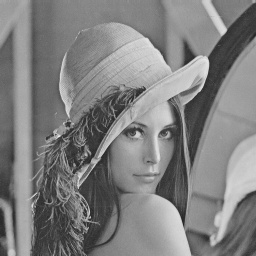
\includegraphics[height=2.5in]{image.jpg}&

\includegraphics[height=2.5in]{Otsus.jpg}\\
input image & Otsu’s thresholding method
\end{tabular}
\end{figure}

\item[•]
{\bf Experience:}\\
Otsu's thresholding method 精神在於群內最小變異、群間最大變異。而再找尋$t$的過程,需求取最大值。我們目前都採取暴力法計算,而我想到一個天馬行空的想法,可以先找Histogram中具有代表性的點進行多項式的插值,然後再用積分取代$\sum$來計算,這樣就可以將問題轉成求分式函數的最大值,最後用Gradient decent來求取t的近似值(以上純屬我的想法,沒有實作過XD)。
\end{enumerate}










\end{document}